\documentclass{article}
\usepackage[utf8]{inputenc}
\usepackage{graphicx}
\usepackage{fancyhdr}
\usepackage[margin=1.8cm]{geometry}
\usepackage{array, multirow}
\usepackage{longtable}
\usepackage{amssymb}
\usepackage{enumitem} % For customizing itemize lists
\usepackage{tabularx}
\usepackage{tikz}
\usepackage{dashrule}
\usepackage[most]{tcolorbox}
\usepackage{booktabs}
\usepackage{mdframed}
\usepackage{adjustbox}
\usepackage{pgf-pie} % pie charts
\usepackage{caption}
\usepackage[bottom]{footmisc}
\usepackage[table]{xcolor}
\usepackage{xcolor}
\usepackage{wrapfig}
\usepackage{titling}
\usepackage{floatrow}
\usepackage{sidecap}



\title{Technical Edge: Daily Range Expansion Model}
\author{\textbf{MR5OBOT} \\ \small{Mentor \& Concept Credits: Michael J. Huddeston}}
\date{\today}

\renewcommand{\maketitle}{%
  \begin{center}
    \vspace*{\fill}
    {\huge\bfseries\thetitle\par}
    \vspace{1.5cm}
    {\Large\theauthor\par}
    \vspace{1cm}
    % {\large\thedate\par}
    \vspace*{\fill}
  \end{center}
}

\begin{document}
\maketitle

\newtcolorbox{notebox}{
    colback=gray!7,
    colframe=gray!0,
    arc=0mm,
    boxrule=0mm,
    left=5mm,
    right=5mm,
    top=1mm,
    bottom=1mm,
}

\renewcommand{\thefootnote}{}
\footnote{Twitter [ @MR-5OBOT ]}
\vspace{0.8cm}

\begin{figure}[h]
  \begin{minipage}{.5\textwidth}
    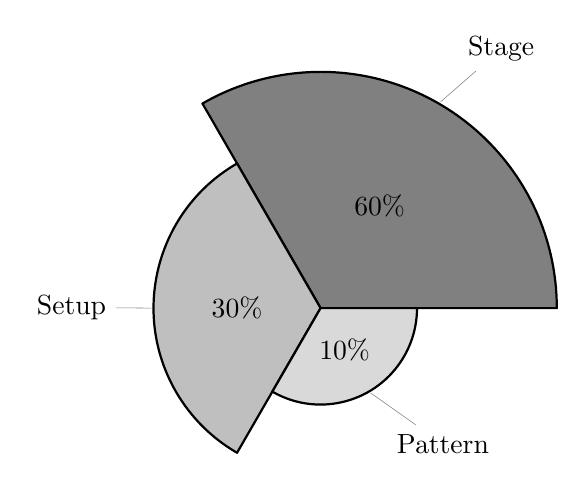
\begin{tikzpicture}[scale=1]
      \pie[polar,text=pin, color={gray!100, gray!50, gray!30}]{60/Stage, 30/Setup, 10/Pattern}
    \end{tikzpicture}
  \end{minipage}
  \begin{minipage}{.45\textwidth}
    \centering
    \section{Model Clarification}
    The following model system is designed to be applied and analyzed in the specific order of : \\
    \vspace{0.5cm}
    HTF = Stage (Narrative)\\
    \vspace{0.2cm}
    MTF = Setup (PDA) \\
    \vspace{0.2cm}
    LTF = Pattern (Entry Model)\\
    \vspace{0.2cm}
    \subsection{Model Objective}
    Intraday focus: capturing the obvious SSL/BSL.
  \end{minipage}
\end{figure}
\vspace{1.5cm}


\begin{table}[h!]
\centering
\definecolor{lightgray}{gray}{0.95}
\renewcommand{\arraystretch}{1}
\setlength{\tabcolsep}{25pt}
\rowcolors{2}{lightgray}{}
\begin{tabular}{|c|c|c|}
  \hline
  \multirow{2}{*}{\textbf{STAGE}} & \multirow{2}{*}{\textbf{SETUP}} & \multirow{2}{*}{\textbf{PATTERN}} \\
   & & \\
  \hline
  Daily Range Expansion & \rule{0pt}{60pt}FVG - OB - HIGHs/LOWs\rule[-60pt]{0pt}{0pt} & \-  The Entry Model  \- \\
  \hline
\end{tabular}
% \caption{The Trade Logs}
\end{table}
\newpage

\section{Higher Timeframe}
The stage for the model is based on indentifying the higherst probability direction and draw for the expansion of the daily candle

\vspace{0.6cm}


\begin{figure}[h]
\begin{minipage}{0.58\textwidth}
\subsection{Identify:}
  \vspace{0.3cm}
  \begin{itemize}
    \item Daily \& Weekly Order flow
    \item Weekly Profiles [day of week]
    \item Daily Profiles [PO3 \& session character]
  \end{itemize}
  \vspace{0.4cm}
$ \rightarrow $ When {\color[HTML]{008000}Bullish,} you are anticipating Open to Low, \\ then expansion toward higher prices \\\\
$ \rightarrow $ When {\color[HTML]{BB5153}Bearish,} you are anticipating Open to High, \\ then expansion towards lower prices

\end{minipage}
\hfill
\begin{minipage}{0.29\textwidth}
  \includegraphics[scale=0.6]{$HOME/Pictures/latex/OHLC.png}
\end{minipage}
\end{figure}
\vspace{0.5cm}

\subsection{Weekly Profiles Provide Context for Expansions}
\begin{SCfigure}[0.2][h]
\begin{minipage}{0.56\textwidth}
\large{$ \rightarrow $ {\color[HTML]{68528D}I.E:} Monday/ Tuesday LOTW, sets up for\\ Wednesday and Thursday Expansions  \\\\\\
$ \rightarrow $ {\color[HTML]{68528D}I.E:} Wednesday/ Thursday low of the Week,\\ sets up for Thursday/ friday Expansions \\\\\\
$ \rightarrow $ {\color[HTML]{68528D}I.E:} Thursday low of the Week,\\ sets up for friday Expansion}
\end{minipage}

\begin{minipage}{0.4\textwidth}
    \centering
    \includegraphics[width=0.8\textwidth]{~/Pictures/latex/W-p.png}
    % \caption{Your caption}
\end{minipage}
\end{SCfigure}

\footnote{Twitter [ @MR-5OBOT ]}
\newpage

\subsection{Daily Profiles Provide Narrative for Expansions}
\vspace{.5cm}
\begin{itemize}
  \item London Reversal
  \item New York Manipulation
  \item New York Reversal
\end{itemize}
\begin{figure}[h]
    \centering
    \begin{minipage}{0.42\textwidth}
        \includegraphics[width=1\textwidth]{~/Pictures/latex/LO-r.png}
    \end{minipage}
    \begin{minipage}{0.42\textwidth}
        \includegraphics[width=1\textwidth]{~/Pictures/latex/Ny-mani.png}
    \end{minipage}
    \begin{minipage}{0.42\textwidth}
        \includegraphics[width=1\textwidth]{~/Pictures/latex/judas.png}
    \end{minipage}
\end{figure}
\footnote{Twitter [ @MR-5OBOT ]}

\newpage
\section{The Setup}
\vspace{0.3cm}
\subsection{HTF PD Arrays}

\vspace{0.3cm}
\begin{itemize}
      \item Order Block
      \item Fair Value Gap
      \item Highs / Lows
\end{itemize}

\vspace{.1cm}
\subsection{The Entry Model}
\vspace{.3cm}

\begin{enumerate}
    \item Liquidity Above/ Below Daily open or HTF PDA engagement
    \item 15M/ 5M [ CISD/ IFVG Formation at Liquidity or PDA Level ] 
    \item 2R Room from Entry point to the next Target
    \item The Most Important Rule, We need to Target the most obvious SSL/ BSL.
\end{enumerate}

\vspace{1cm}
\begin{figure}[h!]
  \begin{center}
  % \caption{London Reversal $\rightarrow$ LHOD}
\begin{adjustbox}{width=1.1\textwidth,center}
  \includegraphics{~/Pictures/latex/diagram.png}
\end{adjustbox}
  \end{center}
\end{figure}
\footnote{Twitter [ @MR-5OBOT ]}
\newpage


\centering \subsection{Chart Examples}

\begin{figure}[h!]
  % \caption{London Reversal $\rightarrow$ LHOD}
\begin{adjustbox}{width=1.15\textwidth,center}
  \includegraphics{~/Pictures/latex/Entry Model-2.png}
\end{adjustbox}
  \label{fig:image}
\end{figure}

\begin{figure}[h!]
  % \caption{New York Reversal $\rightarrow$ NHOD}
\begin{adjustbox}{width=1.15\textwidth,center}
  \includegraphics{~/Pictures/latex/Entry Model-1.png}
\end{adjustbox}
  \label{fig:image}
\end{figure}

\begin{figure}[h!]
  % \caption{New York Reversal $\rightarrow$ NHOD}
\begin{adjustbox}{width=1.15\textwidth,center}
  \includegraphics{~/Pictures/latex/I.E.png}
\end{adjustbox}
  \label{fig:image}
\end{figure}

\begin{figure}[h!]
  % \caption{New York Reversal $\rightarrow$ NHOD}
\begin{adjustbox}{width=1.15\textwidth,center}
  \includegraphics{~/Pictures/latex/I.E2.png}
\end{adjustbox}
  \label{fig:image}
\end{figure}


\footnote{Twitter [ @MR-5OBOT ]}



\end{document}
